\chapter{Group Velocity, Fermionic Exclusion, and the Dirac Sea}

\section{Phase Velocity and Group Velocity}

\begin{classroomqa}
\lecturetimestamp{00:00:07}
\audiencequestion{What are group velocity and phase velocity?}
\lecturerresponse{Phase velocity follows a point of fixed phase in a plane wave. It generally does not describe the motion of a measurable object. Group velocity follows the envelope of a wave packet and is the velocity associated with particles, signals, and probability flow.}
\end{classroomqa}

Begin with a plane wave,
\begin{equation}
\psi(x,t)=e^{i(kx-\omega t)},
\end{equation}
or with its real form,
\begin{equation}
\psi(x,t)=\sin(kx-\omega t).
\end{equation}
A crest, a trough, or any other point of fixed phase moves so that
\begin{equation}
kx-\omega t=\text{constant}.
\end{equation}
Choosing the constant to be zero for convenience gives
\begin{equation}
x=\frac{\omega}{k}t,
\qquad
v_{\mathrm{phase}}=\frac{\omega}{k}.
\end{equation}
Since \(\omega=2\pi/T\) and \(k=2\pi/\lambda\),
\begin{equation}
v_{\mathrm{phase}}=\frac{\omega}{k}=\frac{\lambda}{T}.
\end{equation}
This is just the distance by which a given phase advances during one period.

For a nonrelativistic Schr\"odinger wave, with \(\hbar=1\), energy and momentum are \(\omega\) and \(k\), so
\begin{equation}
\omega(k)=\frac{k^2}{2m}.
\end{equation}
Its phase velocity is therefore
\begin{equation}
v_{\mathrm{phase}}=\frac{k}{2m}.
\end{equation}
The ordinary velocity of a particle with momentum \(k\), however, is \(k/m\). The factor-of-two mismatch is the first warning that the movement of a plane-wave phase is not the movement of the particle.

There is an even sharper warning. Add the same constant \(C\) to every frequency:
\begin{equation}
\omega(k)\longrightarrow \omega(k)+C.
\end{equation}
The constant could, for example, represent a common rest-energy contribution such as \(mc_{\mathrm{light}}^2\), but its particular name is unimportant. Here \(C\) is an energy offset, not the speed of light. The phase velocity changes to
\begin{equation}
v_{\mathrm{phase}}\longrightarrow
\frac{\omega(k)+C}{k}
=v_{\mathrm{phase}}+\frac{C}{k}.
\end{equation}
Yet adding the same constant to every energy changes no energy difference and hence no nonrelativistic physics.

This can be seen directly in the wavefunction. Write a general Schr\"odinger field as a sum or integral of modes,
\begin{equation}
\psi(x,t)=\sum_k a_k e^{ikx}e^{-i\omega(k)t},
\end{equation}
with normalization factors suppressed. After the shift,
\begin{align}
\psi(x,t)
&\longrightarrow
\sum_k a_k e^{ikx}e^{-i[\omega(k)+C]t}
\\
&=e^{-iCt}\psi(x,t).
\end{align}
Every mode has acquired the same time-dependent phase. The conjugate field acquires the opposite phase, and therefore
\begin{equation}
\begin{aligned}
\psi^*(x,t)\psi(x,t)
&\longrightarrow
e^{iCt}e^{-iCt}\psi^*(x,t)\psi(x,t)
\\
&=\psi^*(x,t)\psi(x,t).
\end{aligned}
\end{equation}
The same cancellation occurs in expectation values. A quantity that changes when the zero of energy is shifted cannot be the physical propagation speed of the Schr\"odinger particle. Phase velocity is therefore partly conventional.

A localized particle is represented not by one infinite plane wave but by a packet. The component waves add constructively in the region of the packet and destructively outside it. The motion of this pattern can already be found from two nearby waves:
\begin{equation}
\psi(x,t)=
\sin(kx-\omega t)+
\sin(k'x-\omega't),
\end{equation}
where \(k'\) is close to \(k\) and \(\omega'=\omega(k')\). A locus of constructive interference occurs where their phases agree,
\begin{equation}
kx-\omega t=k'x-\omega't.
\end{equation}
Thus
\begin{equation}
(k-k')x=(\omega-\omega')t,
\end{equation}
and the reinforcing pattern moves according to
\begin{equation}
x=\frac{\omega-\omega'}{k-k'}t.
\end{equation}
Taking the neighboring-wave limit gives
\begin{equation}
x=\frac{d\omega}{dk}t,
\qquad
v_{\mathrm{group}}=\frac{d\omega}{dk}.
\end{equation}
This is the velocity of the envelope---the localized lump produced by the interference of the component waves.

For the nonrelativistic dispersion relation, including the arbitrary offset,
\begin{equation}
\omega(k)=\frac{k^2}{2m}+C,
\end{equation}
the group velocity is
\begin{equation}
v_{\mathrm{group}}
=\frac{d}{dk}\left(\frac{k^2}{2m}+C\right)
=\frac{2k}{2m}
=\frac{k}{m}.
\end{equation}
The additive constant has disappeared, and the result is precisely the classical particle velocity.

\begin{classroomqa}
\lecturetimestamp{00:16:35}
\audiencequestion{Does the factor of two disappear in the group velocity?}
\lecturerresponse{Yes. Differentiating \(k^2\) produces \(2k\), which cancels the two in \(2m\). The result is \(k/m\).}
\end{classroomqa}

Group velocity is consequently the velocity most closely associated with classical particle motion. It is also the velocity relevant to the propagation of a packet and, in the ordinary circumstances considered here, to the propagation of signals. Phase velocity need not have either meaning.

\subsection{Massless and Massive Relativistic Waves}

\begin{classroomqa}
\lecturetimestamp{00:17:47}
\audiencequestion{Does this have to do with claims that light can travel faster than light?}
\lecturerresponse{No. Those claims raise a separate issue. A related calculation does show that a phase can move faster than light while the physical group velocity remains subluminal, but that does not describe a signal outrunning light.}
\end{classroomqa}

\begin{classroomqa}
\lecturetimestamp{00:18:05}
\audiencequestion{Is the relevant example the familiar one in which phase velocity exceeds the speed of light while group velocity remains below it?}
\lecturerresponse{Yes. The same pattern appears for a relativistic wave with nonzero mass, and it follows directly from the relativistic energy--momentum relation.}
\end{classroomqa}

Set \(\hbar=c_{\mathrm{light}}=1\). The relativistic relation is
\begin{equation}
E=\sqrt{p^2+m^2},
\qquad
\omega(k)=\sqrt{k^2+m^2}.
\end{equation}
It is useful to establish the massless case first. When \(m=0\),
\begin{equation}
\omega=|k|.
\end{equation}
On the right-moving branch \(k>0\), \(\omega=k\), and therefore
\begin{equation}
v_{\mathrm{phase}}=\frac{\omega}{k}=1,
\qquad
v_{\mathrm{group}}=\frac{d\omega}{dk}=1.
\end{equation}
On the left-moving branch both velocities have the corresponding negative sign. In either case their speed is the speed of light. Because the dispersion relation is linear on either branch, all Fourier components on that branch move with the same velocity.

For a massive particle with \(k>0\),
\begin{equation}
v_{\mathrm{phase}}
=\frac{\omega}{k}
=\sqrt{\frac{k^2+m^2}{k^2}}>1,
\end{equation}
whereas
\begin{equation}
v_{\mathrm{group}}
=\frac{d\omega}{dk}
=\frac{k}{\sqrt{k^2+m^2}}<1.
\end{equation}
For \(k<0\), both velocities reverse sign, while their magnitudes obey the same inequalities. Thus the phase can move faster than light while the packet, particle, energy, and signal move more slowly than light. For this particular dispersion relation and \(k\neq0\),
\begin{equation}
v_{\mathrm{phase}}v_{\mathrm{group}}=1.
\end{equation}
That inverse relation is an accident of the square-root dispersion relation, not a general property of waves.

\begin{figure}
\centering

\includegraphics[width=0.72\textwidth]{lecture_05_figure_03.png}
\caption{Nonrelativistic and relativistic dispersion relations, with phase velocity \(\omega/k\) and group velocity \(d\omega/dk\).}
\lectureframe{00:35:52}
\end{figure}

\begin{classroomqa}
\lecturetimestamp{00:23:41}
\audiencequestion{Is dispersion tied to the wave speed depending on frequency?}
\lecturerresponse{Yes. When \(\omega(k)\) is linear, every Fourier component has the same group velocity and a packet can retain its shape. When \(\omega(k)\) is nonlinear, different components move at different velocities, so the packet disperses and changes shape. Low-frequency sound is approximately nondispersive when its frequency is nearly proportional to wave number.}
\end{classroomqa}

Phase velocity ordinarily carries neither signal nor energy nor probability flow. Its numerical value can even be changed by shifting the zero of energy. The group velocity is the physically relevant motion of a sufficiently narrow packet.

\begin{classroomqa}
\lecturetimestamp{00:25:14}
\audiencequestion{Can phase velocity be measured for a photon?}
\lecturerresponse{In vacuum a photon has linear dispersion, so its phase and group velocities coincide and both equal the speed of light. In a material medium the dispersion relation changes, and phase and group velocities need not agree.}
\end{classroomqa}

\begin{classroomqa}
\lecturetimestamp{00:25:50}
\audiencequestion{Is this discussion restricted to wave packets that do not spread with time?}
\lecturerresponse{A packet remains nonspreading only when all of its Fourier components share one velocity, which corresponds to a linear dispersion relation over the relevant range. With nonlinear dispersion the components separate and the packet spreads.}
\end{classroomqa}

Questions about light cones and relativistic causal structure require more than the distinction between phase and group velocity and are left separate from this calculation.

\section{Translation Symmetry and Conservation Laws}

The same plane-wave phases give a compact account of conservation laws. Begin with energy conservation. An annihilation field acting on an incoming particle of energy \(\omega_j\) contributes a time factor
\begin{equation}
e^{-i\omega_j t},
\end{equation}
whereas a creation field producing an outgoing particle of energy \(\omega'_r\) contributes
\begin{equation}
e^{+i\omega'_r t}.
\end{equation}
For several incoming and outgoing particles, their product is
\begin{equation}
\exp\!\left[
i\left(\sum_r\omega'_r-\sum_j\omega_j\right)t
\right].
\end{equation}
If the interaction may occur at any time with the same amplitude, the amplitude includes an integral over the interaction time:
\begin{equation}
\begin{aligned}
&\int_{-\infty}^{\infty}dt\,
\exp\!\left[
i\left(\sum_r\omega'_r-\sum_j\omega_j\right)t
\right]
\\
&\quad =2\pi\,
\delta\!\left(\sum_r\omega'_r-\sum_j\omega_j\right).
\end{aligned}
\end{equation}
The delta function requires total outgoing energy to equal total incoming energy. Equal amplitude at every possible interaction time is time-translation invariance, and it produces energy conservation.

Space translation gives momentum conservation by the same mechanism. Consider a physical one-to-two decay in which an incoming particle of momentum \(k\) disappears and two particles of momenta \(k'_1\) and \(k'_2\) appear. A local interaction at position \(x\) contains one annihilation field and two creation fields,
\begin{equation}
\mathcal{O}(x)=\psi^\dagger(x)\psi^\dagger(x)\psi(x).
\end{equation}
Suppressing time dependence and normalization, the relevant mode factors are
\begin{align}
\psi(x)&\supset a_k e^{ikx},
\\
\psi^\dagger(x)&\supset a_{k'_1}^\dagger e^{-ik'_1x},
\qquad
\psi^\dagger(x)\supset a_{k'_2}^\dagger e^{-ik'_2x}.
\end{align}
In the matrix element
\begin{equation}
\langle k'_1,k'_2|\mathcal{O}(x)|k\rangle,
\end{equation}
the annihilation operator removes the incoming particle and the two creation operators supply the outgoing particles. Once those operator actions are taken, the position-dependent factor that remains is
\begin{equation}
e^{-ik'_1x}e^{-ik'_2x}e^{ikx}
=e^{i(k-k'_1-k'_2)x}.
\end{equation}
Because no position is privileged, one integrates over all possible decay positions:
\begin{equation}
\int_{-\infty}^{\infty}dx\,
e^{i(k-k'_1-k'_2)x}
=2\pi\delta(k-k'_1-k'_2).
\end{equation}
The surviving amplitude therefore obeys
\begin{equation}
k=k'_1+k'_2.
\end{equation}
In three dimensions the same calculation uses \(d^3x\), bold momentum vectors, and a three-dimensional delta function. Nothing in the argument depends on having only one incoming particle or two outgoing particles. For arbitrary particle numbers, integration over the common interaction position produces
\begin{equation}
\delta^{(3)}\!\left(
\sum_j\mathbf{k}_j-\sum_r\mathbf{k}'_r
\right).
\end{equation}
Equal amplitude at every position is spatial translation invariance, and it gives momentum conservation just as equal amplitude at every time gives energy conservation.

A third example is a global phase rotation,
\begin{equation}
\psi\longrightarrow e^{i\lambda}\psi,
\qquad
\psi^\dagger\longrightarrow e^{-i\lambda}\psi^\dagger.
\end{equation}
An interaction amplitude is invariant when the phases contributed by its annihilation and creation fields cancel. For a field carrying electric charge, this equality of charge removed from the initial state and restored in the final state is charge conservation. Thus time translations, space translations, and global phase rotations illustrate how fields that create and annihilate particles encode energy, momentum, and charge conservation.

\begin{classroomqa}
\lecturetimestamp{00:37:52}
\audiencequestion{Does integration over space mean integration over all three spatial dimensions?}
\lecturerresponse{Yes. The three integrations produce a delta function for the three momentum components, so all three components of total momentum are conserved.}
\end{classroomqa}

\begin{classroomqa}
\lecturetimestamp{00:38:03}
\audiencequestion{Does this model determine the relative probabilities for different ways of sharing the conserved momentum?}
\lecturerresponse{No. This simple expression enforces the sum of the outgoing momenta but is otherwise neutral about their division. Relative probabilities require additional dynamical information.}
\end{classroomqa}

\begin{classroomqa}
\lecturetimestamp{00:39:04}
\audiencequestion{Why does a sum of annihilation operators reduce to the term matching the occupied momentum?}
\lecturerresponse{An annihilation operator acting on an empty mode gives the zero vector. If the state contains one particle only in the mode \(k_0\), every term except the one with \(k=k_0\) vanishes.}
\end{classroomqa}

For example,
\begin{equation}
\sum_k a_k e^{ikx}|1_{k_0}\rangle
=e^{ik_0x}|0\rangle,
\end{equation}
up to normalization: all annihilators associated with empty modes return the zero vector.

\section{Bosonic Enhancement and Fermionic Exclusion}

Bosons permit any nonnegative occupation number in a one-particle state, and their creation-operator algebra actually favors an already occupied state. For one bosonic mode, the normalized number-state convention writes the occupation enhancement as\footnote{The lecture states the square-root occupation enhancement; this indexed equation is its standard number-state form.}
\begin{equation}
a^\dagger|n\rangle=\sqrt{n+1}\,|n+1\rangle.
\end{equation}
Suppose an excited atom can emit a photon into many possible modes. In the absence of other photons, the different directions and momenta occur with their ordinary probability distribution. If a particular mode already contains many photons---all with the same momentum, energy, and frequency---emission into that mode is enhanced by the corresponding square-root occupation factor. The atom preferentially adds its photon to the state already populated. This is stimulated emission and is a concrete expression of bosonic congregation.

Fermions behave in the opposite way. Two identical fermions cannot occupy the same quantum state. The exclusion principle first arose in atomic physics, where two electrons in an atom cannot have identical quantum numbers, but it is not confined to atoms: identical fermions cannot share a complete one-particle state anywhere.

The field expansion initially looks just like the bosonic one. In a finite box one may write
\begin{equation}
\psi(x)=\sum_k A_k e^{ikx},
\qquad
\psi^\dagger(x)=\sum_k A_k^\dagger e^{-ikx}.
\end{equation}
For continuous momentum the sums become integrals. The opposite sign in the conjugate spatial phase follows from Hermitian conjugation. This part of the construction is nonrelativistic; relativistic fermions will enter only at the end.

The state of the field is still recorded by an occupation number for every mode, but now each number can only be zero or one:
\begin{equation}
|n_{k_1},n_{k_2},\ldots\rangle,
\qquad n_k\in\{0,1\}.
\end{equation}
There are no additional relativistic particle types with, say, at most three particles per state or at least seven particles per state. Establishing that bosonic and fermionic statistics are the only possibilities requires quantum mechanics together with special relativity and lies beyond the present discussion. Here the task is to describe the fermionic possibility and its consequences.

\subsection{One Fermionic State}

Focus on a single one-particle state. It is either empty, \(|0\rangle\), or occupied, \(|1\rangle\). Creation and annihilation act as
\begin{align}
A^\dagger|0\rangle&=|1\rangle,
&
A^\dagger|1\rangle&=0,
\\
A|0\rangle&=0,
&
A|1\rangle&=|0\rangle.
\end{align}
The unadorned zero on the right is the zero vector, not the empty state \(|0\rangle\). Attempting to add a second fermion does not return the vacuum; it returns no physical state at all.

\begin{classroomqa}
\lecturetimestamp{00:46:25}
\audiencequestion{Are the fermionic creation and annihilation operators still linear?}
\lecturerresponse{Yes. Quantum-mechanical operators are linear operators, including the fermionic creation and annihilation operators.}
\end{classroomqa}

\begin{classroomqa}
\lecturetimestamp{00:47:34}
\audiencequestion{Does zero mean the empty state, or does it mean that the attempted operation cannot produce a state?}
\lecturerresponse{It means the zero vector, not the empty state. A genuine vacuum or ground state has a nonzero wavefunction; the identically zero function has zero norm and is not a physical state.}
\end{classroomqa}

The harmonic oscillator makes the distinction concrete. Its ground state, the state with no oscillator excitation, has a Gaussian wavefunction such as
\begin{equation}
\phi_0(q)\propto e^{-\alpha q^2},
\qquad \alpha>0.
\end{equation}
This is a perfectly good, normalizable state. By contrast,
\begin{equation}
\phi(q)\equiv0
\end{equation}
is the zero vector: it has no probability amplitude anywhere and is not a state. Thus \(A^\dagger|1\rangle=0\) says that the attempted second creation produces the zero vector.

\begin{classroomqa}
\lecturetimestamp{00:48:42}
\audiencequestion{Should fermion operators use notation different from boson operators?}
\lecturerresponse{Yes. It is clearer to reserve \(a\) and \(a^\dagger\) for bosonic modes and use \(c\) and \(c^\dagger\) for fermionic modes. Both conventions occur in the literature, but different letters keep the two algebras distinct.}
\end{classroomqa}

Adopting that notation, the single-mode rules are
\begin{align}
c^\dagger|0\rangle&=|1\rangle,
&c^\dagger|1\rangle&=0,
\\
c|0\rangle&=0,
&c|1\rangle&=|0\rangle.
\end{align}
Now evaluate the two possible products on both basis states. On the empty state,
\begin{align}
c^\dagger c|0\rangle&=0,
&
cc^\dagger|0\rangle&=|0\rangle.
\end{align}
On the occupied state,
\begin{align}
c^\dagger c|1\rangle&=|1\rangle,
&
cc^\dagger|1\rangle&=0.
\end{align}
Their sum returns whichever state it acts on:
\begin{align}
(c^\dagger c+cc^\dagger)|0\rangle&=|0\rangle,
\\
(c^\dagger c+cc^\dagger)|1\rangle&=|1\rangle.
\end{align}
Since \(|0\rangle\) and \(|1\rangle\) span the one-mode state space,
\begin{equation}
c^\dagger c+cc^\dagger=1.
\end{equation}
The plus-sign combination is the anticommutator,
\begin{equation}
\{A,B\}=AB+BA,
\end{equation}
so the fermionic relation is
\begin{equation}
\{c,c^\dagger\}=1.
\end{equation}
It is the fermionic analog of the bosonic commutator
\begin{equation}
[a,a^\dagger]=aa^\dagger-a^\dagger a=1.
\end{equation}

Two creations in the same fermionic state always vanish. If the state is empty, the first creation fills it and the second fails; if it is already occupied, the first creation already fails. Similarly, two annihilations always vanish. Therefore
\begin{equation}
\{c^\dagger,c^\dagger\}=2(c^\dagger)^2=0,
\qquad
\{c,c\}=2c^2=0.
\end{equation}

\begin{classroomqa}
\lecturetimestamp{00:56:45}
\audiencequestion{Is the zero in the squared-annihilation relation a zero vector?}
\lecturerresponse{The equation states that \(c^2\) is the zero operator. It is an operator that sends every state vector to the zero vector. The zero operator and the zero vector are different mathematical objects, although the former always produces the latter.}
\end{classroomqa}

For many discrete momentum modes, the full algebra is
\begin{align}
\{c_k,c_{k'}^\dagger\}&=\delta_{kk'},
\\
\{c_k,c_{k'}\}&=0,
\\
\{c_k^\dagger,c_{k'}^\dagger\}&=0.
\end{align}
The Kronecker delta is one when \(k=k'\) and zero otherwise. For continuous momenta it is replaced, with the appropriate normalization, by a Dirac delta function. The same-type anticommutators vanish for every pair of modes, not only when their labels coincide.

\subsection{Exclusion in Position Space}

The momentum-labeled algebra first says that two identical fermions of the same species cannot occupy one momentum mode. It says more. A particle localized at position \(x\) is created by
\begin{equation}
\psi^\dagger(x)=\sum_k c_k^\dagger e^{-ikx},
\end{equation}
up to normalization. At the origin, trying to create two particles gives
\begin{align}
\psi^\dagger(0)\psi^\dagger(0)|\Omega\rangle
&=\sum_{k,k'}c_k^\dagger c_{k'}^\dagger|\Omega\rangle.
\end{align}
The labels \(k\) and \(k'\) are dummy summation variables. Interchanging them leaves the double sum unchanged, so it may be averaged with its relabeled form:
\begin{align}
\sum_{k,k'}c_k^\dagger c_{k'}^\dagger|\Omega\rangle
&=\frac12\sum_{k,k'}
\left(c_k^\dagger c_{k'}^\dagger
+c_{k'}^\dagger c_k^\dagger\right)|\Omega\rangle
\\
&=\frac12\sum_{k,k'}
\{c_k^\dagger,c_{k'}^\dagger\}|\Omega\rangle
=0.
\end{align}

\begin{classroomqa}
\lecturetimestamp{01:02:26}
\audiencequestion{Do only terms with unequal momenta vanish in the two-particle position-state sum?}
\lecturerresponse{No. Relabeling the dummy indices turns the whole double sum into one half of the anticommutator of two creation operators. That anticommutator vanishes for every pair of momenta, so the complete sum is zero.}
\end{classroomqa}

The calculation shows that exclusion is not peculiar to momentum eigenstates. Identical fermions cannot be placed in the same position state either. More generally, they cannot occupy any identical one-particle state.

\subsection{What Constitutes the Same State?}

\begin{classroomqa}
\lecturetimestamp{01:04:30}
\audiencequestion{Can two far-separated electrons have the same momentum?}
\lecturerresponse{Exclusion concerns the complete one-particle state. Two electrons can have the same exact momentum eigenvalue when another commuting label, such as spin, differs. Spatially separated electrons are instead localized packets rather than exact momentum eigenstates; their mean momenta can be nearly equal while their spatial wavefunctions remain distinct. What is forbidden is equality of the complete states.}
\end{classroomqa}

Spin has not yet been developed, but it supplies a familiar additional label. Two electrons can share the same momentum value when their spin states differ. Once every relevant label is included, no two identical fermions may share the same full state.

\begin{classroomqa}
\lecturetimestamp{01:05:25}
\audiencequestion{Can electrons in two separated hydrogen atoms have the same momentum or atomic state?}
\lecturerresponse{An electron bound in an atom is not a momentum eigenstate. Its orbital wavefunction is centered on that atom. Two separated atoms may each have an electron in what is called the atomic ground state, but one orbital is centered at the first atom and the other at the second, so they are different one-particle states.}
\end{classroomqa}

\begin{classroomqa}
\lecturetimestamp{01:06:33}
\audiencequestion{Can the more general word system replace state?}
\lecturerresponse{No. A system is a collection of degrees of freedom; a state specifies a particular quantum configuration of that system. An electron is a system, while its orbital and spin wavefunction describes a state of that system.}
\end{classroomqa}

\begin{figure}
\centering

\includegraphics[width=0.74\textwidth]{lecture_05_figure_04.png}
\caption{Localized one-particle wavefunctions and the two-creation-operator state used to test fermionic exclusion.}
\lectureframe{01:07:21}
\end{figure}

\begin{classroomqa}
\lecturetimestamp{01:07:22}
\audiencequestion{Does an electron stream in a cathode-ray tube contain no two electrons in the same state?}
\lecturerresponse{Yes. The electrons occupy distinct wave packets, separated in position or otherwise distinguished in their full states. This contrasts with photons, which may all occupy the same plane-wave mode and build a coherent beam.}
\end{classroomqa}

An electron beam can be pictured as one localized packet followed by another. The packets need not be exact position states or exact momentum states; it is enough that their wavefunctions are distinct. A photon beam, by contrast, may have many photons in precisely the same plane-wave state.

\begin{classroomqa}
\lecturetimestamp{01:08:14}
\audiencequestion{Can two electrons be at the same position with different momenta?}
\lecturerresponse{Exact position and exact momentum are incompatible labels because the corresponding operators do not commute. One cannot specify a one-particle state by simultaneously sharp position and momentum. Spin can accompany a position or momentum label because spin commutes with those observables in this nonrelativistic setting.}
\end{classroomqa}

\begin{classroomqa}
\lecturetimestamp{01:08:51}
\audiencequestion{Are separated bound electrons approximately in position states?}
\lecturerresponse{They are not exact position eigenstates, because each orbital has finite spatial extent, but each is approximately localized near its own atom. That localization is enough to make the two orbital wavefunctions different states.}
\end{classroomqa}

\begin{classroomqa}
\lecturetimestamp{01:09:31}
\audiencequestion{What is the definition of a quantum state?}
\lecturerresponse{A state is the quantum analog of a system's configuration. It contains the information needed to assign probabilities to the possible measurements. For one electron, the state is represented by a wavefunction, together with any internal labels such as spin.}
\end{classroomqa}

\begin{classroomqa}
\lecturetimestamp{01:10:32}
\audiencequestion{Can electrons localized in very distant places be in the same state or have the same momentum?}
\lecturerresponse{They cannot be the same state because their localization differs: an electron here and one in the Andromeda Galaxy, or one in Nevada and one in Connecticut, have distinct wavefunctions. They may have nearly equal momenta. Making either momentum infinitely sharp would spread the corresponding wavefunction through space and destroy the localization that distinguished the states.}
\end{classroomqa}

The standard-deviation form of the position--momentum uncertainty relation is\footnote{The lecture gives the qualitative uncertainty-product statement; the factor \(\hbar/2\) is supplied in the standard-deviation convention.}
\begin{equation}
\Delta x\,\Delta p\geq\frac{\hbar}{2}.
\end{equation}
A packet can be localized in Nevada and have a fairly narrow momentum distribution, while another packet in Connecticut has nearly the same distribution. They remain different states because their spatial wavefunctions differ. In the exact momentum-eigenstate limit, neither packet remains localized in either place.

Fermion operators are used in reactions in the same way as bosonic operators. An electron annihilation operator removes an incoming electron, an electron creation operator supplies an outgoing electron, and these factors can be multiplied by photon creation or annihilation operators. Photons are bosons, while electrons are fermions. Products of their operators provide the bookkeeping for reactions involving incoming and outgoing electrons together with emitted or absorbed photons.

\begin{classroomqa}
\lecturetimestamp{01:13:36}
\audiencequestion{Is Pauli exclusion locally communicated, or is it globally enforced when two creation processes are spatially separated?}
\lecturerresponse{If one particle is known to be in Nevada and the other in Connecticut, then they are not in the same state.}
\end{classroomqa}

\editorialnote{A short portion of the reply to this question is not recoverable. The distinction between localized one-particle states and the Nevada--Connecticut superpositions is secure.}

When their locations are not definite, exclusion asks whether the full one-particle wavefunctions coincide. The Nevada--Connecticut superpositions make that distinction explicit.

Let \(|N\rangle\) and \(|C\rangle\) be orthonormal states localized in Nevada and Connecticut. Then
\begin{equation}
|+\rangle=\frac{|N\rangle+|C\rangle}{\sqrt2},
\qquad
|-\rangle=\frac{|N\rangle-|C\rangle}{\sqrt2}.
\end{equation}
The state \(|+\rangle\) gives equal probabilities of finding its one electron in Nevada or Connecticut. The state \(|-\rangle\) gives the same position probabilities but differs by a relative phase. The two states are orthogonal:
\begin{equation}
\langle+|-\rangle=0.
\end{equation}
Two electrons cannot both occupy \(|+\rangle\), and they cannot both occupy \(|-\rangle\), but exclusion does not prevent one electron from occupying each state.

\begin{classroomqa}
\lecturetimestamp{01:16:25}
\audiencequestion{Can one electron occupy the plus Nevada--Connecticut superposition and another the minus superposition?}
\lecturerresponse{Yes. The plus and minus combinations are orthogonal and therefore distinct one-particle states.}
\end{classroomqa}

\begin{classroomqa}
\lecturetimestamp{01:16:39}
\audiencequestion{Does the separated-state example require a notion of simultaneity?}
\lecturerresponse{The present model is nonrelativistic. It compares the two occupied states on one common time slice, with an absolute time shared by the spatially separated Nevada and Connecticut regions. It also ignores finite-speed operational limitations on comparing those regions. Relativistic physics introduces additional fuzziness in how particles are localized without undoing exclusion, but that refinement is postponed here.}
\end{classroomqa}

The essential nonrelativistic statement is now fixed: fermions are described by anticommuting creation and annihilation operators, and no two identical fermions can occupy one complete one-particle state. The many-body ground state therefore differs radically from that of bosons.

\section{Bosonic and Fermionic Ground States in a Finite Box}

Consider particles confined to a finite three-dimensional box of side \(L\), with periodic boundary conditions. In one dimension the allowed wave numbers are
\begin{equation}
k=\frac{2\pi n}{L},
\qquad n\in\mathbb{Z}.
\end{equation}
In three dimensions this condition applies component by component:
\begin{equation}
\mathbf{k}=\frac{2\pi}{L}(n_x,n_y,n_z),
\qquad n_x,n_y,n_z\in\mathbb{Z}.
\end{equation}
The allowed momentum vectors therefore form a lattice in momentum space. This is not a lattice of positions; each point labels an allowed momentum state. Increasing \(L\) decreases the separation \(2\pi/L\) between neighboring values, while the lattice continues without bound in every momentum direction.

\begin{figure}
\centering
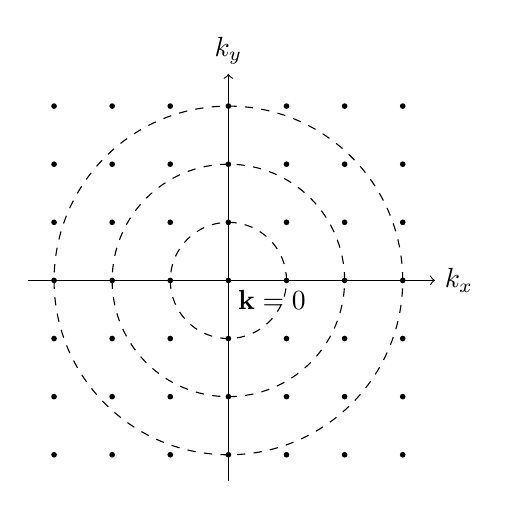
\begin{tikzpicture}[scale=0.82]
\draw[->] (-3.1,0) -- (3.2,0) node[right] {$k_x$};
\draw[->] (0,-3.1) -- (0,3.2) node[above] {$k_y$};
\draw[dashed] (0,0) circle (0.9);
\draw[dashed] (0,0) circle (1.8);
\draw[dashed] (0,0) circle (2.7);
\foreach \x in {-3,-2,-1,0,1,2,3}{
  \foreach \y in {-3,-2,-1,0,1,2,3}{
    \fill (0.9*\x,0.9*\y) circle (1.25pt);
  }
}
\node[below right] at (0,0) {$\mathbf{k}=0$};
\end{tikzpicture}
\caption{Discrete momentum states and constant-energy shells for particles in a finite periodic box.}
\end{figure}

For a nonrelativistic particle,
\begin{equation}
E_{\mathbf{k}}=\frac{\mathbf{k}^2}{2m},
\end{equation}
so the state of lowest energy is \(\mathbf{k}=0\). Put \(N\) identical bosons in the box and seek the many-particle ground state. The first boson goes into the zero-momentum state. The second can go into the same state, as can the third and every subsequent boson. Thus all \(N\) bosons occupy \(\mathbf{k}=0\).

This is a boson condensate: a large number of identical particles occupying the same one-particle state, here the lowest-energy state. The zero-momentum wavefunction is spatially constant and extends throughout the box. It does not localize any one boson at a particular position; each boson is correspondingly uncertain about where it is. When the occupation becomes large, the common wavefunction builds up a macroscopic field amplitude, and the field behaves increasingly like a classical field.

The fermionic ground state is entirely different. Ignore spin for the moment, so that each momentum point represents one available state. The first fermion goes into \(\mathbf{k}=0\), but a second identical fermion cannot join it. The next particles must occupy the next-lowest energy shell. In a two-dimensional drawing there are four nearest nonzero lattice points of equal energy; in three dimensions there are six. After those states are occupied, further particles must enter successive shells.

Because the energy is proportional to the squared distance from the origin in momentum space, minimizing the total energy means packing the occupied points as closely around \(\mathbf{k}=0\) as exclusion permits. With many fermions the occupied region approximates a sphere. Its boundary is the Fermi surface, its interior is the Fermi sea, and the complete filled region is the Fermi sphere. At finite volume the boundary is slightly jagged because the available points form a lattice, but this detail becomes negligible for a large system.

\begin{figure}
\centering
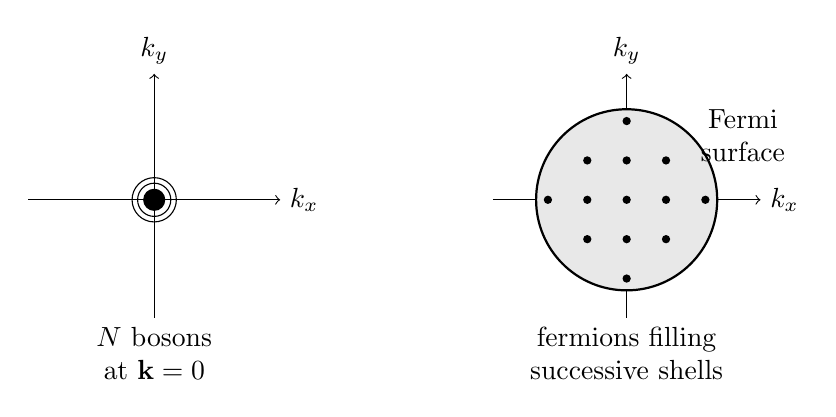
\begin{tikzpicture}[scale=1.0]
\begin{scope}[xshift=-3.0cm]
\draw[->] (-1.6,0) -- (1.6,0) node[right] {$k_x$};
\draw[->] (0,-1.5) -- (0,1.6) node[above] {$k_y$};
\fill (0,0) circle (4pt);
\draw (0,0) circle (6pt);
\draw (0,0) circle (8pt);
\node[align=center] at (0,-1.95) {$N$ bosons\\at $\mathbf{k}=0$};
\end{scope}
\begin{scope}[xshift=3.0cm]
\draw[->] (-1.7,0) -- (1.7,0) node[right] {$k_x$};
\draw[->] (0,-1.5) -- (0,1.6) node[above] {$k_y$};
\fill[gray!18] (0,0) circle (1.15);
\draw[thick] (0,0) circle (1.15);
\fill (0,0) circle (1.5pt);
\fill (0.5,0) circle (1.5pt);
\fill (-0.5,0) circle (1.5pt);
\fill (0,0.5) circle (1.5pt);
\fill (0,-0.5) circle (1.5pt);
\fill (0.5,0.5) circle (1.5pt);
\fill (0.5,-0.5) circle (1.5pt);
\fill (-0.5,0.5) circle (1.5pt);
\fill (-0.5,-0.5) circle (1.5pt);
\fill (1,0) circle (1.5pt);
\fill (-1,0) circle (1.5pt);
\fill (0,1) circle (1.5pt);
\fill (0,-1) circle (1.5pt);
\node[right,align=center] at (0.82,0.82) {Fermi\\surface};
\node[align=center] at (0,-1.95) {fermions filling\\successive shells};
\end{scope}
\end{tikzpicture}
\caption{Bosons condense into the zero-momentum state, whereas fermions fill momentum states outward to a Fermi surface.}
\end{figure}

The fermionic ground state has much more energy than the corresponding bosonic ground state. All the bosons can remain at zero momentum, but most of the fermions are forced into nonzero-momentum states. As more fermions are added, the maximum occupied momentum grows. Moreover, a shell at large momentum contains more lattice points than a shell near the origin. A large Fermi sphere therefore contains many particles at substantial momentum and only a small number in the lowest-momentum states.

The contrast continues in the excited states. For bosons, the first excitation is obtained by removing any one boson from the condensate and placing it in a first excited one-particle state:
\begin{equation}
(N,0,0,\ldots)\longrightarrow (N-1,1,0,\ldots).
\end{equation}
It makes no difference which boson is moved; the particles are identical. Higher excitations can be made in several ways. Depending on the level spacing, one may place one boson in a higher level or place two bosons in the first excited level. Exciting the bosonic system means promoting particles out of the condensate into higher-energy states.

For fermions, no particle can be moved to another point inside the filled Fermi sphere, because every such point is already occupied. Taking a fermion from deep inside the sea and placing it above the surface is possible, but it costs a large amount of energy. The least expensive excitation takes a fermion from just inside the Fermi surface and moves it to an unoccupied state just outside. The promoted electron has only a small energy above the surface, and the vacant state left behind lies only a small energy below it.

\begin{figure}
\centering
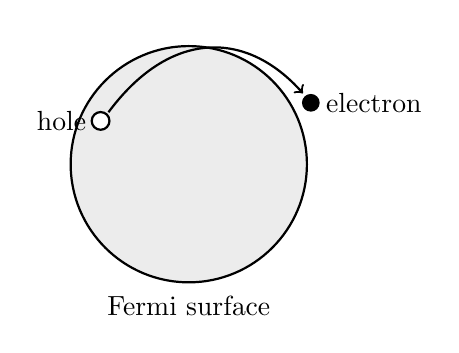
\begin{tikzpicture}[scale=1.0]
\fill[gray!15] (0,0) circle (1.5);
\draw[thick] (0,0) circle (1.5);
\draw[fill=white,thick] (-1.12,0.55) circle (3.2pt);
\fill (1.55,0.78) circle (3.2pt);
\draw[->,thick] (-1.02,0.66) .. controls (-0.25,1.7) and (0.72,1.72) .. (1.45,0.9);
\node[left] at (-1.18,0.55) {hole};
\node[right] at (1.62,0.78) {electron};
\node[below] at (0,-1.55) {Fermi surface};
\end{tikzpicture}
\caption{A low-energy fermionic excitation promotes an electron through the Fermi surface and leaves a hole behind.}
\end{figure}

\section{Holes and Low-Energy Excitations}

To make the charge of the hole concrete, imagine that the box contains positive charge uniformly smeared through its volume. In matter that positive charge ultimately comes from protons in nuclei, but the uniform distribution keeps the model simple. Add enough electrons to neutralize the background. In the ground state those electrons fill the Fermi sphere.

Promoting one electron from below to above the Fermi surface does not change the total charge of the box. It creates a negatively charged electron above the surface and leaves a missing negative charge below it. The missing electron can therefore be treated as a positively charged excitation: a hole.

\begin{classroomqa}
\lecturetimestamp{01:31:38}
\audiencequestion{Does a hole below the Fermi surface have negative energy?}
\lecturerresponse{No. A hole is an excitation above the many-body ground state, so its excitation energy is positive. Removing an occupied electron from below the Fermi surface costs a positive amount of energy when energies are measured relative to that surface.}
\end{classroomqa}

Let the removed electron have energy \(\varepsilon<\varepsilon_F\), and let the promoted electron have energy \(\varepsilon'>\varepsilon_F\). The energy supplied may be separated into two positive distances from the Fermi surface.\footnote{The two intervals are stated separately; the compact equality displayed here is the algebraically equivalent reconstruction.}
\begin{equation}
\Delta E
=\varepsilon'-\varepsilon
=(\varepsilon'-\varepsilon_F)+(\varepsilon_F-\varepsilon).
\end{equation}
The first contribution is naturally assigned to the electron above the Fermi surface, while the second is assigned to the hole below it:
\begin{equation}
E_{\mathrm{electron}}=\varepsilon'-\varepsilon_F>0,
\qquad
E_{\mathrm{hole}}=\varepsilon_F-\varepsilon>0.
\end{equation}
The electron carries negative charge, and the hole carries positive charge.

An electron above the Fermi surface may later drop into an available hole. Its energy then decreases, so radiation must carry the released energy away. One may describe the event as an electron dropping to an unoccupied lower state and emitting one or more photons. Equivalently, one may say that an electron and a hole annihilate into radiation. The hole is not an additional fundamental constituent of the box; it is an absence in the filled many-electron state. Nevertheless, its energy and charge make it useful to treat it as a particle-like excitation.

\begin{classroomqa}
\lecturetimestamp{01:36:52}
\audiencequestion{Does promoting an electron mean moving it from one lattice point to another in momentum space?}
\lecturerresponse{It means moving the electron from one energy level to another. For free particles in the box, the momentum lattice labels those levels, but the same idea does not depend on a momentum-space lattice. In an atom the positive charge is concentrated in the nucleus. Electrons fill the lowest available atomic levels, and a photon can promote one electron to an excited level, leaving a vacancy in the level from which it came. That vacancy is the atomic counterpart of a hole.}
\end{classroomqa}

In the box, photon absorption likewise converts the photon energy into an electron above the Fermi surface and a hole below it. In an atom, the same language describes the excited electron together with the vacancy left among the occupied lower levels.

\begin{classroomqa}
\lecturetimestamp{01:39:16}
\audiencequestion{Can a low-energy photon be absorbed by an electron anywhere in the Fermi sphere?}
\lecturerresponse{No. If the electron lies deep in the Fermi sea, every nearby state is already occupied, and a low-energy photon cannot lift it all the way to an unoccupied state above the surface. Only electrons close enough to the Fermi surface have accessible empty states within the photon's energy range. A sufficiently energetic photon can excite an electron from deep in the sea.}
\end{classroomqa}

The low-energy absorption cross section is therefore controlled by the surface of the Fermi sea rather than by its whole volume. Electrons deep in the sea are blocked from making small transitions; electrons just below the surface can be moved just above it.

\begin{classroomqa}
\lecturetimestamp{01:40:42}
\audiencequestion{What prevents electrons from interacting directly with one another, without an incident photon?}
\lecturerresponse{Nothing. Electron--electron interactions are being neglected in this simple model, because including them makes the Fermi-sea picture more complicated. In this first approximation to a metal, their effective influence is treated as weak enough that it can usually be ignored.}
\end{classroomqa}

\begin{classroomqa}
\lecturetimestamp{01:41:10}
\audiencequestion{What happens if one photon carries enough energy to excite several electrons?}
\lecturerresponse{Any process consistent with the conservation laws is possible in principle. The photon can create more than one electron--hole pair: exciting two electrons also leaves two holes. Such a process creates more excitations and is generally less probable than using the energy to excite one electron much more strongly.}
\end{classroomqa}

\begin{classroomqa}
\lecturetimestamp{01:42:06}
\audiencequestion{Can two photons be absorbed together when neither photon alone can produce the excitation?}
\lecturerresponse{Yes. Absorption is probabilistic, and a two-photon process can occur when the combined photon energy reaches an available excitation even though either photon separately falls below the required energy. If the available light carries too little energy to reach any allowed excitation, it largely passes through the system.}
\end{classroomqa}

\editorialnote{A brief discussion at this point connects absorbed radiation with collective electron motion, but its substantive details are not recoverable. Only the statement that such collective response is more complicated than the single particle--hole picture is secure.}

\begin{classroomqa}
\lecturetimestamp{01:43:49}
\audiencequestion{Why are electron--electron interactions called weak when all electrons carry the same negative charge?}
\lecturerresponse{The electrons are immersed in the compensating positive background. That background screens the charge of an electron and reduces the effective interaction in this simplified setting. The interaction is not absent; treating it requires the screening response of the medium.}
\end{classroomqa}

\begin{classroomqa}
\lecturetimestamp{01:44:41}
\audiencequestion{Will screening be discussed later?}
\lecturerresponse{Yes. Screening is important, but it is deferred until the interacting system can be treated more fully.}
\end{classroomqa}

\section{A One-Dimensional Fermionic Sea and Antiparticles}

The hole construction points toward antiparticles. The same logical structure can be transferred from electrons in matter to a relativistic quantum field and its vacuum. The simplest version uses one spatial dimension and a massless fermionic field \(\psi(x,t)\). In units with the speed of light equal to one, the two possible linear dispersion relations are
\begin{equation}
\omega=k,
\qquad\text{or}\qquad
\omega=-k.
\end{equation}
The first branch will be considered explicitly.

\editorialnote{The closing exchange alternates incompatible particle identifications. The secure model is an unspecified massless fermionic toy field in one spatial dimension, restricted to one direction of propagation.}

For a plane wave
\begin{equation}
\psi(x,t)=e^{i(kx-\omega t)},
\end{equation}
the derivatives are
\begin{equation}
\frac{\partial\psi}{\partial t}=-i\omega\psi,
\qquad
\frac{\partial\psi}{\partial x}=ik\psi.
\end{equation}
Thus \(\omega=k\) is equivalent to the first-order field equation
\begin{equation}
\frac{\partial\psi}{\partial t}
=-\frac{\partial\psi}{\partial x}.
\end{equation}

\begin{figure}
\centering

\includegraphics[width=0.72\textwidth]{lecture_05_figure_05.png}
\caption{Beginning the first-order field equation whose plane waves satisfy \(\omega=k\).}
\lectureframe{01:47:22}
\end{figure}

Any profile of the form \(f(x-t)\) satisfies this equation and moves to the right. Reversing the sign gives
\begin{equation}
\frac{\partial\psi}{\partial t}
=+\frac{\partial\psi}{\partial x},
\end{equation}
whose profiles \(f(x+t)\) move to the left. Either first-order equation selects only one direction of motion. Take the field to be fermionic and, for the hole argument, suppose that its particles carry electric charge.

The branch \(\omega=k\) contains an immediate difficulty. The wave number \(k\) can be negative, and therefore so can \(\omega\). Since \(\omega\) is the energy in these units, the straight-line spectrum contains both positive- and negative-energy states:
\begin{equation}
E=\omega=k.
\end{equation}

\begin{figure}
\centering
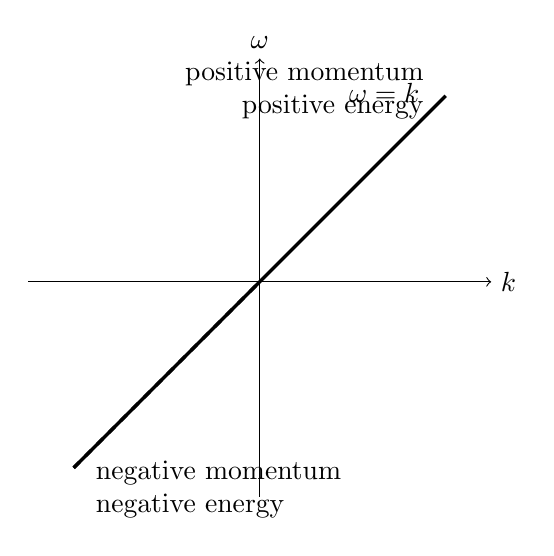
\begin{tikzpicture}[scale=1.05]
\draw[->] (-2.8,0) -- (2.8,0) node[right] {$k$};
\draw[->] (0,-2.6) -- (0,2.7) node[above] {$\omega$};
\draw[very thick] (-2.25,-2.25) -- (2.25,2.25);
\draw[very thick,dashed] (-2.25,-2.25) -- (0,0);
\node[above left] at (2.05,2.05) {$\omega=k$};
\node[below right,align=left] at (-2.1,-2.05) {negative momentum\\negative energy};
\node[above left,align=right] at (2.1,1.85) {positive momentum\\positive energy};
\end{tikzpicture}
\caption{The one-branch spectrum \(\omega=k\), with its negative-energy half at \(k<0\).}
\end{figure}

An ordinary empty vacuum cannot be the ground state of such a theory. A positive-energy fermion could radiate a photon and fall to a lower state. Nothing would force it to stop at zero: it could continue into states of negative energy, emit still more radiation, and fall without bound. The energy lost by the fermion would appear in the radiation field. A spectrum unbounded below therefore gives no stable ordinary vacuum.

Fermionic exclusion supplies a different starting point. Fill every negative-energy one-particle state, up to zero energy, with one fermion. No further fermion can fall into those states because each is already occupied. Adding another negative-energy fermion is impossible, while adding a positive-energy fermion raises the energy. The completely filled negative-energy sea can therefore be taken as the many-body ground state and called the vacuum.

\begin{figure}
\centering
\resizebox{\linewidth}{!}{%
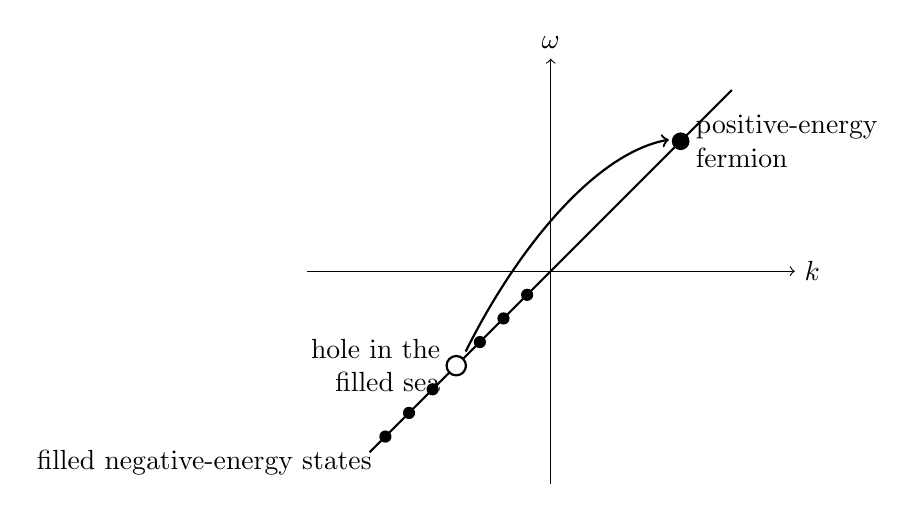
\begin{tikzpicture}[scale=1.0]
\draw[->] (-3.1,0) -- (3.1,0) node[right] {$k$};
\draw[->] (0,-2.7) -- (0,2.7) node[above] {$\omega$};
\draw[thick] (-2.3,-2.3) -- (2.3,2.3);
\foreach \p in {-2.1,-1.8,-1.5,-1.2,-0.9,-0.6,-0.3}{
  \fill (\p,\p) circle (2.2pt);
}
\draw[fill=white,thick] (-1.2,-1.2) circle (3.5pt);
\fill (1.65,1.65) circle (3.2pt);
\draw[->,thick] (-1.08,-1.02) .. controls (-0.45,0.25) and (0.55,1.5) .. (1.5,1.67);
\node[left,align=right] at (-1.28,-1.2) {hole in the\\filled sea};
\node[right,align=left] at (1.72,1.65) {positive-energy\\fermion};
\node[below left] at (-2.15,-2.15) {filled negative-energy states};
\end{tikzpicture}%
}
\caption{The filled negative-energy sea and an excitation formed by promoting one fermion to positive energy.}
\end{figure}

The simplest excitation removes one fermion from the negative-energy sea and places it in a positive-energy state. The promoted fermion is an ordinary positive-energy particle. The vacancy left in the sea is a second excitation, a hole. If the removed fermion has negative charge, the hole has positive charge.

The hole also has positive momentum in this one-branch example. If the missing fermion occupied a state of momentum \(k_-<0\), removing it changes the total momentum by
\begin{equation}
p_{\mathrm{hole}}=-k_->0.
\end{equation}
It is a deficit of negative momentum. Thus the excitation consists of a positive-energy, negatively charged fermion and a positive-energy, positively charged hole. Both carry positive momentum and, on the \(\omega=k\) branch, both move to the right.

In the full electron theory, the positively charged hole is the positron. Dirac initially considered identifying the hole with the proton. The construction requires a particle and its antiparticle to have the same mass. The hole is a distinct particle with the electron's mass and the opposite electric charge. This is the basic particle--antiparticle interpretation to which the negative-energy spectrum led.

The same rescue cannot be applied to bosons. A bosonic state admits arbitrarily many particles, so there is no way to fill a negative-energy level once and block further occupation. More bosons could always be added to that level, lowering the energy again and again:
\begin{equation}
\begin{aligned}
\text{fermionic mode: }&n=0\ \text{or}\ 1,\\
\text{bosonic mode: }&n=0,1,2,\ldots .
\end{aligned}
\end{equation}
The proposed bosonic system would still have no ground state. In this elementary construction, the stability of the filled sea depends precisely on fermionic exclusion.

This one-dimensional equation is only a toy version of the Dirac equation. Its field is massless, moves at the speed of light, and propagates in only one direction. A fuller Dirac equation must accommodate the missing directions of motion and the rest of the relativistic particle structure. That fuller equation, together with the treatment of antiparticles for bosonic fields, is postponed.
